\documentclass[article]{memoir}
\renewcommand{\cftchapterdotsep}{\cftdotsep}% Chapters should use dots in ToC
\let\subsubsection\subsection
\let\subsection\section % undo article option change of divisions
\let\section\chapter    % ditto
\usepackage{xcolor}
\usepackage[utf8]{inputenc}
\usepackage{array}
\usepackage{ragged2e}
\usepackage[portuguese]{babel}
\usepackage{emoji}
\usepackage[nolist]{acronym}
\usepackage{float}
\usepackage{caption}
\footnotesinmargin % set footnotes in the margin
\usepackage{graphicx}
\usepackage{makeidx}
\usepackage{tcolorbox}
\usepackage{enumitem}
\setlist[enumerate]{label*=\arabic*.}
\usepackage{fancyhdr}
\usepackage{tikz}
\usetikzlibrary{shapes.geometric, arrows}
\usepackage{subcaption}
\usepackage{caption}
\newcounter{run}
\InputIfFileExists{\jobname.runs}{}{}
\stepcounter{run}

\usepackage{atveryend}
\usepackage{newfile}
\AtVeryEndDocument{%
	\newoutputstream{runs}%
	\openoutputfile{\jobname.runs}{runs}%
	\addtostream{runs}{\string\setcounter{run}{\number\value{run}}}%
	\closeoutputstream{runs}%
}



\pagestyle{fancy}
\fancyhf{} % clear all fields
\fancyhead[L]{\rightmark}
\fancyhead[R]{\thepage}

\renewcommand{\subsectionmark}[1]{%
	\markright{\MakeUppercase{\thesubsection.\ #1}}}%




\newcommand*\lowercasecapitals[1]{\MakeLowercase{\large\scshape#1}}
\setsecheadstyle{\lowercasecapitals}


\usepackage[hyperpageref]{backref}
\usepackage{listings}
\renewcommand{\lstlistingname}{Código}
\usepackage{xcolor}
\usepackage{ifpdf}
%\ifpdf
%\pdfinfo{
	%	/Author (Cledson de Sousa)
	%	/Title  (Apostila de Geência de Redes e Engenharia de Tráfego)
	%	/CreationDate (D:20240407)
	%	/Subject (Gerência de Redes e Engenharia de Tráfego)
	%	/Keywords (Tráfego e redes)
	%}
%\fi
\usepackage{multicol}
\usepackage{hyperref}
\hypersetup{
	pdftitle={Arquitetura de Sistemas Computacionais para Telecomunicações},
	pdfsubject={Switches e Roteadores},
	pdfauthor={Prof.: Cledson de Sousa},
	pdfkeywords={switches e roteadores}
	%pdfdate = {april 07, 2024}
}

\setcounter{secnumdepth}{3}

% Definição das cores no estilo GitHub
\definecolor{backcolour}{rgb}{0.95, 0.95, 0.92}
\definecolor{codegreen}{rgb}{0,0.6,0}
\definecolor{codeblue}{rgb}{0.24, 0.37, 0.78}
\definecolor{codegray}{rgb}{0.5, 0.5, 0.5}
\definecolor{codepurple}{rgb}{0.58, 0, 0.82}
\definecolor{magenta}{rgb}{1.0, 0.0, 1.0}



\makeindex % Inicializa o sistema de índice remissivo



\begin{document}
	
% Estilo de listagem no estilo GitHub
\lstdefinestyle{github}{
	backgroundcolor=\color{backcolour},   
	commentstyle=\color{magenta},       % Define a cor dos comentários como verde
	keywordstyle=\color{codeblue},
	numberstyle=\tiny\color{codegray},
	stringstyle=\color{codepurple},
	basicstyle=\ttfamily\footnotesize,
	breakatwhitespace=false,         
	breaklines=true,                 
	captionpos=b,                    
	keepspaces=true,                 
	numbers=left,                    
	numbersep=5pt,                  
	showspaces=false,                
	showstringspaces=false,
	showtabs=false,                  
	tabsize=2,
	morecomment=[l]{\%}
	morecomment=[l]{;}
	              % Define o símbolo de comentário como "%"
}
\lstset{style=github}

%\cite{abntex2classe}
% Capa

	\begin{titlingpage} % Ambiente para a capa
		\centering
		\vspace*{1cm}
		\Huge Universidade Federal Fluminense \\
		%\Large Apostila de Gerência de Redes e Engenharia de Tráfego
		\vspace{2cm}
		% Espaço reservado para figura/logo
		\vspace{1cm} % Ajuste este espaço conforme necessário
		
\includegraphics[width=0.8\textwidth]{figs/uffdataacademy.png}
		% Descomente a linha acima e substitua "caminho-para-sua-figura-aqui.png" pelo caminho correto do arquivo de imagem que você deseja incluir
		
		\vspace{1cm}
		\Huge \textbf{Gerência de Redes e Engenharia de Tráfego}\\[0.5cm] % Título

		
		\vfill
		\Large Professor Cledson de Sousa\\[0.5cm] % Seu nome
		Versão: 0.1.\therun -- 13 de maio/2024 -- Até MPLS.
		%Data do Curso: \today % Ou coloque a data específica
		

		
	\end{titlingpage}	
\setcounter{secnumdepth}{4}
\setcounter{tocdepth}{4}
	\tableofcontents*



%\section*{Lista de Acrônimos}

\begin{acronym}
%\begin{multicols}{2}
	\begin{footnotesize}
	\acro{AAL}[AAL]{\textit{Adaptation Layer}} 
	\acro{ATM}[ATM]{\textit{Asynchronous Transfer Mode}}
	\acro{BGP}[BGP]{\textit{Border Gateway Protocol}}
	\acro{DevOps}[DevOps]{\textit{Development and Operations}}
	\acro{ET}[ET]{Engenharia de Tráfego}
	\acro{FCAPS}[FCAPS]{\textit{Fault, Configuration, Accounting, Performance, and Security}}
	\acro{IGP}[IGP]{\textit{Interior Gateway Protocol}}
	\acro{IP}[IP]{\textit{Internet Protocol}}
	\acro{IETF}[IETF]{\textit{Internet Engineering Task Force}}
	\acro{MPLS}[MPLS]{\textit{Multiprotocol Label Switching}}
	\acro{NFV}[NFV]{\textit{Network Functions Virtualization}}
	\acro{RFC}[RFC]{\textit{Request for Comments}}
	\acro{TE}[TE]{Traffic Engineering}
	\acro{QoS}[QoS]{\textit{Quality of Service}}
	\acro{SDN}[SDN]{\textit{Software-Defined Networking}}
	\acro{SLA}[SLA]{\textit{Service Level Agreement}}
	\acro{VLAN}[VLAN]{\textit{Virtual Local Area Network}}
	\acro{VPN}[VPN]{\textit{Virtual Private Network}}
\end{footnotesize}
%\end{multicols}
\end{acronym}

\section*{Prefácio}

Caros futuros engenheiros, 

Bem-vindos ao curso de Gerência de Redes e Engenharia de Tráfego, uma disciplina  criada para introduzir os conceitos fundamentais e práticas avançadas da controle de tráfego. administração e gerência de modernas infraestruturas de rede. Este curso, estruturado com uma mistura equilibrada de aulas em classe e extra-classe, cobre uma carga horária total de 60 horas, das quais 40 horas são dedicadas a conceitos teóricos e 20 horas a aplicações fora de sala. Então o objetivo é proporcionar aos alunos uma compreensão abrangente dos modelos de gerência de redes, monitoramento, auditoria e a engenharia de tráfego necessária para lidar com o encaminhamento do tráfego.


Esta apostila, embora tenha um caráter acadêmico, não possui a pretensão de ser extremamente rigorosa, especialmente na forma. O autor empenhou-se em dar o devido crédito a todas as fontes utilizadas; no entanto,por vezes, estende-se o texto sem as devidas citações específicas dos autores originais. Então peço que aceitem as escusas do autor, pois muitas das fontes são os textos originais presentes nos locais onde as figuras foram extraídas. Além disso, diversas explicações são fruto do esforço do autor em dissecar os diagramas, que frequentemente simplificam o verdadeiro encaminhamento dos pacotes.

Ao longo do texto há diversos sinais de parada \emoji{stop-sign}, em notas de margem, gráficos, figuras e outros sinais. Estes sinais lá estão  para o leitor desopilar, se você chegou em um desses sinais parabéns! É por que você já leu o suficiente, nesse momento é bom parar, descontrair, visitar os sites e sair um pouco do texto, naturalmente deve-se retornar ao texto tão logo possível. Essa estratégia funciona comigo!
Um curso leve, produtivo, enriquecedor e sem reprovações. É o que desejo!

\textbf{Sobre o autor:}

O autor recebeu seu título de Doutor em Computação pela Universidade Federal Fluminense (UFF) em 2019, e seus títulos de graduação e mestrado em Engenharia de Telecomunicações pela mesma universidade, em 1997 e 2013. Com mais de 30 anos de experiência na indústria de telecomunicações, desde 2021 é Professor Adjunto do Departamento de Engenharia de Telecomunicações da Universidade Federal Fluminense. Seus interesses de pesquisa atuais incluem redes de sensores sem fio, SDN, rádios cognitivos e CSI.\mbox{}\\

\textbf{Plataformas:}

\begin{itemize}
	\item LinkedIn: \url{https://www.linkedin.com/in/cledsonsousa}
	\item Página pessoal: \url{https://cledsonsousa.github.io}
	\item Currículo Lattes: \url{http://lattes.cnpq.br/7195080748145566}
\end{itemize}

\newpage

\section{O Conceito de Camadas}
O conceito de camadas (\textit{layering}) é fundamental para a visualização de dados, Vamos explorar como esse conceito facilita essas representações:

\paragraph*{Separação de Elementos Visuais:}\mbox{}\\
Camadas permitem separar diferentes elementos visuais em uma visualização de dados. Por exemplo, ao representar um conjunto de dados, uma camada pode ser usada para mostrar os valores médios, enquanto outra camada pode ser usada para mostrar a variação desses valores (como barras de erro ou intervalos de confiança). Isso ajuda a distinguir claramente entre os dados principais e as informações auxiliares que podem por exemplo  representar incerteza.

\paragraph*{Flexibilidade na Visualização:}\mbox{}\\
O uso de camadas oferece flexibilidade na criação de gráficos complexos. Diferentes tipos de representações visuais, como pontos de dados, linhas de tendência, e intervalos de confiança, podem ser adicionados ou removidos conforme necessário. Isso permite que os visualizadores ajustem a complexidade da visualização com base em suas necessidades específicas.

\begin{figure}[ht]
	\centering
	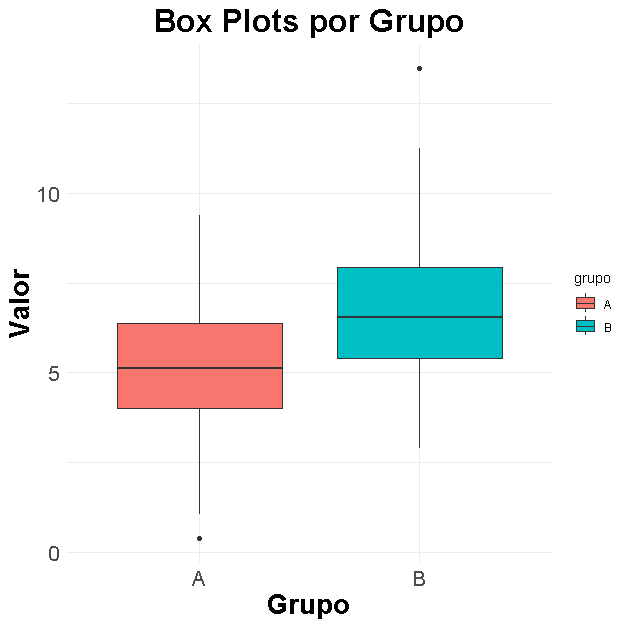
\includegraphics[width=0.5\linewidth]{figs/layers_box_plt_example}
	\caption{}
	\label{fig:layersboxpltexample}
\end{figure}


\paragraph*{Exemplo Prático:}\mbox{}\\
 \textit{Box plots} como o apresentados na Figura 	\ref{fig:layersboxpltexample}, por exemplo, utilizam camadas. A camada do \textit{box plot} mostra a mediana e os quartis, enquanto camadas adicionais indicam \textit{outliers}.


	
\section{Variação e Incertezas}


O conceito de camadas também facilita a representação da variação estatística e da incerteza. É importante se lembrar que dados experimentais tipicamente apresentam alguma incerteza  e a visualização e representação destes dados deve "caracterizar a magnitude dessa incerteza em relação aos dados reais  \cite{wainer1996depicting}. 

Os autores infelizmente mostram resultados que em muitos trabalhos as figuras publicadas não atendem a esse padrão, especialmente à medida que a dimensionalidade dos dados aumenta \cite{allen2012data}. Quando o objetivo de uma visualização é comparar uma quantidade medida ou derivada entre categorias ou condições, deve-se incluir um elemento (são as \textit{geom} do \texttt{ggplot}) gráfico retratando a quantidade e um segunda elemento  retratando a incerteza da quantidade. Note que, sem a representação da incerteza, uma comparação visual precisa não é possível, os leitores podem tirar conclusões incorretas ou mal informadas.

A variação e a incerteza podem ser retratadas com uma variedade de \textit{geoms}, mas são mais comumente exibidas com barras de erro. Infelizmente, não há um padrão único para o que a barra de erro deve representar já que há uma pluralidade esmagadora de significados possíveis, como desvio padrão (DP) da amostra, erro padrão da média (EPM), Intervalo de Confiança (IC) paramétrico de $100(1 − \alpha)\%$ , intervalo de probabilidade bayesiano, um intervalo de previsão, etc. Cada quantidade tem sua própria interpretação estatística

Portanto, ao usar barras de erro, certifique-se de que (1) a quantidade codificada pela barra é consistente com o objetivo da visualização e (2) a quantidade é definida de forma inequívoca. Em relação ao primeiro ponto, oferecemos as seguintes diretrizes ao usar barras de erro para retratar a variação de uma estimativa de parâmetro ou a variação dos dados.
\begin{figure}[ht]
	\centering
	\begin{minipage}{0.7\textwidth} % Ajuste a largura total da figura aqui
		\begin{subfigure}[b]{0.45\textwidth}
			\centering
			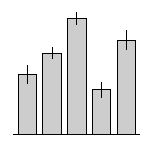
\includegraphics[width=\textwidth]{figs/error_bar_example}
			\caption{Gráficos de barra com barra de erros.}
			\label{fig:sub1}
		\end{subfigure}
		\hfill
		\begin{subfigure}[b]{0.45\textwidth}
			\centering
			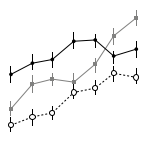
\includegraphics[width=\textwidth]{figs/error_line_example}
			\caption{Gráficos de linhas com barra de erros.}
			\label{fig:sub2}
		\end{subfigure}
	\end{minipage}
	\caption{as barras normalmente para comparar categorias e as linhas para comparar grupos e tendências.}
	\label{fig:ex_bar_lines}
\end{figure}

Se o interesse for estimar um parâmetro populacional, como a média ou a variância, então a variação da estimativa (isto é, a distribuição amostral da estatística) é desejada. Exemplos de barras de erro adequadas incluem o EPM ou um IC paramétrico ou \textit{bootstrap} de 95\%, como visto em visualizações que enfatizam comparações (Figura	\ref{fig:ex_bar_lines}). ICs paramétricos devem ser usados apenas se os dados atenderem às suposições do modelo subjacente, caso contrário, um bootstrap (ou outra estratégia para aproximar a distribuição amostral) deve ser usado\footnote{E o que é $\alpha$? o nível de significância: 
	$\alpha$ é a probabilidade de cometer um erro tipo I, que ocorre quando rejeitamos a hipótese nula ($H_0$)
	 quando ela é verdadeira. \textbf{Em outras palavras, é a taxa de falso positivo permitida.}}. 

\begin{tcolorbox}
	\textbf{IC um conceito muitas vezes mal entendido \cite{belia2005} e \cite{hoekstra2014}}
	
	Um intervalo de confiança de $100(1 − \alpha)\%$  para um parâmetro populacional é um intervalo calculado a partir dos dados amostrais que, em $100(1 − \alpha)\%$ das amostras possíveis, conteria o verdadeiro valor do parâmetro.
	
	\textbf{Isto é:} Suponha que você calcule a média de alturas de uma amostra de 100 pessoas e obtenha uma média de 170 cm com um desvio padrão de 10 cm. Um intervalo de confiança de 95\% pode ser calculado, e você pode obter algo como (168 cm, 172 cm). Isso significa que, se você repetisse esse experimento várias vezes, 95\% dos intervalos de confiança calculados conteriam a verdadeira média populacional (nesse caso 170 cm).
	
\end{tcolorbox} 

Um outro exemplo de interpretação geométrica dos intervalos de confiança são a sua sobreposição ou não entre duas amostras.

\begin{tcolorbox}
	\textbf{A sobreposição dos ICs  \cite{cumming2007} e \cite{krzywinski2013}}
	
	Um intervalo de confiança de $100(1 − \alpha)\%$  para um parâmetro populacional é um intervalo calculado a partir dos dados amostrais que, em $100(1 − \alpha)\%$ das amostras possíveis, conteria o verdadeiro valor do parâmetro.
	
	\textbf{Isto é:} Suponha que você calcule a média de alturas de uma amostra de 100 pessoas e obtenha uma média de 170 cm com um desvio padrão de 10 cm. Um intervalo de confiança de 95\% pode ser calculado, e você pode obter algo como (168 cm, 172 cm). Isso significa que, se você repetisse esse experimento várias vezes, 95\% dos intervalos de confiança calculados conteriam a verdadeira média populacional (nesse caso 170 cm).
	
\end{tcolorbox} 



 Enquanto ICs de 95\% não sobrepostos indicam uma diferença significativa (sob um modelo de probabilidade normal), o inverso não é verdadeiro — dependendo do tamanho da amostra, as barras de IC podem se sobrepor em até 50\% e ainda atender aos critérios de significância.



\begin{figure}[ht]
	\centering
	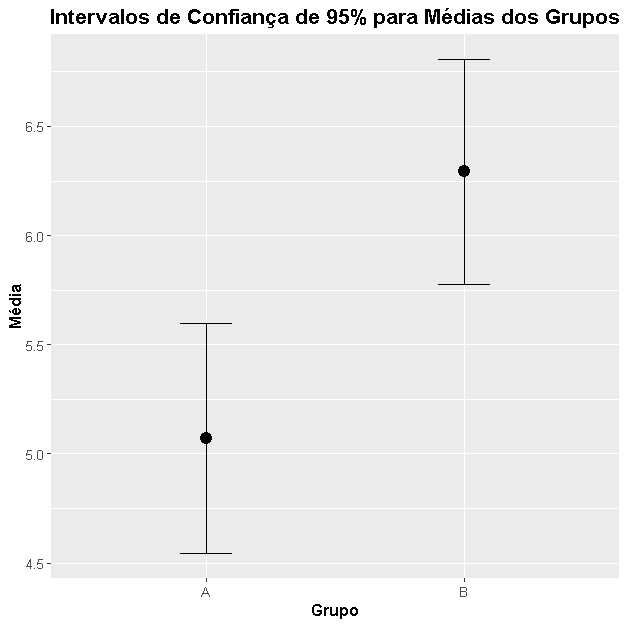
\includegraphics[width=0.7\linewidth]{figs/IC_sobrep_visual}
	\caption{ICs de 95\% não sobrepostos indicam uma diferença significativa (sob um modelo de probabilidade normal).}
	\label{fig:icsobrepvisual}
\end{figure}






\newpage, 
%\pagebreak
\thispagestyle{plain}
\printpagenotes
\bibliographystyle{unsrt}
\bibliography{vis_rep_data.bib}
\thispagestyle{plain}
\end{document}